\section{Contexto}


\subsection{Construcción de interfaces de usuario usando el patrón MVC}
\subsubsection{MVC}

El patrón Modelo Vista Controlador (MVC) es un estilo de arquitectura de
software que separa el modelo de dominio, la interfaz de usuario,
y la relación entre ellos \emph{(Controlador)} en tres componentes distintos.
\cite{burbeck87}

La idea principal de MVC, y que influyó a la mayoria del os frameworks de
presentación posteriores, es la de Presentación Separada \emph{(Separated
Presentation)} que consiste en hacer una división clara entre objetos de 
dominio que modelan nuestra percepción del mundo real y objetos de presentación 
que son los elementos Interfaz de usuarios que vemos en la pantalla. 
Esto nos brinda una clara separación de responsabilidades entre interfaz,
lógica de negocio y de control, además nos permite soportar múltiples
presentaciones para un mismo modelo de datos. \cite{reenskaug79}
  
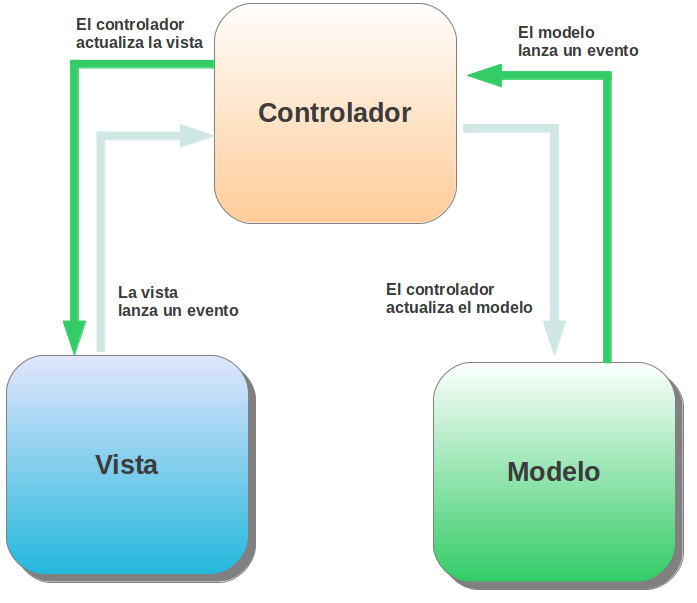
\includegraphics[width=300px, height=300px]{img/mvc}


\begin {itemize}

	\item {\bf Modelo}
		El modelo maneja el comportamiento y los datos del dominio de la aplicación,
		responde a los pedidos de información sobre su estado, 
		y responde a las instrucciones para cambiar su estado. 
		
		
	\item {\bf Vista}
		La Vista muestra la información del modelo al usuario e interactua y recibe
		las acciones.
		
	\item {\bf Controlador}
		Es el intermediario entre el modelo y la vista.
		Captura los eventos emanados tanto del modelo como de la interfaz, y coordina
		la interaccion de ambos.
		

\end {itemize}

\subsubsection{Eventos}

Un evento es un suceso en el sistema (tal como una interacción del usuario con
la máquina, o un mensaje enviado por un objeto).  
El sistema maneja el evento enviando el mensaje adecuado al objeto pertinente. 
También se puede definir como evento, a la reacción que puede desencadenar un objeto,  es decir la acción
que genera. (wiki)

Muchas implementaciones de eventos en el patron mvc, se construyen utilizando el
patron observer \cite{Gamma1995}.\\

{\bf Objetivo:} Definir una dependencia 1:n de forma que cuando el objeto 1
	cambie su estado, los n objetos sean notificados y se actualicen
	automáticamente. Esto me permite tener relaciones entre objetos sin
	acoplamiento.\\

{\bf Motivación:} En la contrucción de interfaces de usuarios, se tirnde
a separar los objetos de presentación (vistas) de los objetos de dominio, de
forma que se puedan tener varias vistas sincronizadas de los mismos datos.\\


Hay MVC's que en su implementación no utilizan eventos: TODO citar.


\subsubsection{Binding}
El binding es una conección de propiedades entre dos objetos. 
Nos permite sincronizar los valores de las propiedades de dos objetos diferentes
(por ejemplo: vista y modelo). Esto se logra a travez de el uso de eventos.
Cada vez que el valor de una propiedad cambia, el objeto notifica (lanza un
evento), y todas las propiedades que estén bindeadas a el reflejan los cambios automáticamente, 
dando la posibilidad de transformar y validar los datos\\
También automatiza el procedimiento de el traspaso de los datos del
modelo a la interfaz y viceversa.


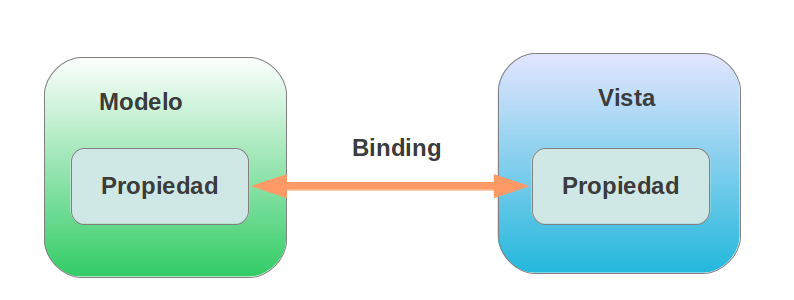
\includegraphics[width=300px]{img/binding}

Al no tener binding perdemos mucho tiempo de desarrollo en  traspasar los
datos de los objetos de dominio hacia los componentes de la interfaz gráfica y
viceversa, repitiendo muchas lineas de código.
Podemos tener datos inconsistentes, como por ejemplo, al mostrarse la interfaz,
muestra el valor actual de la propiedad de un objeto de dominio, y después el
objeto de dominio cambia el valor de su propiedad, la interfaz no se actualiza,
y los datos quedan inconsistentes.

\bigskip

Existen dos implementaciones de binding:

\begin {itemize}

\item {\bf Unidireccional}
Con este tipo de binding el flujo de datos se realiza en una sola dirección.
{Completar más}


\item {\bf Binireccional}
En este tipo de asociación el flujo se produce en ambas direcciones. Los cambios
realizados en el modelo se ven reflejados  en la vista y viceversa. (Este es el
tipo de binding que tenemos en el Arena). Esto es posible, gracias a la
utilización de los eventos, tanto desde el dominio como de la interfaz.
En nuestro trabajo nos enfocamos en este tipo de binding.


\end {itemize}


\subsubsection{Limitationes}
Requiere que mis objetos de dominio, conozcan el concepto de eventos.

Otro problema que aparece frecuentemente es que el binding en su versión más 
sencilla modifica los objetos directamente, por lo que al cancelar una operación 
se debe volver al estado anterior, y este proceso es repetitivo y propenso a errores. 
Con frecuencia implica introducir comportamiento propio de la interfaz de
usuario, en mis objetos de dominio, mezclando la lógica de las dos partes de
la aplicación. Esto me obliga a adaptar mi dominio a este sistema, y repetir
muchas líneas de código.
	
\subsection{Transacciones:}	

Una transacción en un conjunto de órdenes que se ejecutan formando una unidad de
trabajo, es decir, en forma indivisible o atómica.

Una transacción necesita cumplir con un conjunto de características denominadas
{\bf ACID} ({\bf A}tomicity, {\bf C}onsistency, {\bf I}solation and 
{\bf D}urability: Atomicidad, Consistencia, Aislamiento y Durabilidad en
español.)\cite{LA POSTA}

\begin {itemize}

  \item	
  	{\bf Atomicidad:} Todos los cambios en los datos se realizan como si fueran
  	una sola operación.  Es decir, todos se realizan, o ninguno	de ellos, y por
  	lo tanto ante un fallo del sistema no puede quedar a medias.
  
  \item
	{\bf Consistencia:} Sólo se empieza aquello que se puede acabar. Por lo tanto
	se ejecutan aquellas operaciones que no van a romper las reglas y directrices
	de integridad de la base de datos.
  
  \item
	{\bf Aislamiento:} Una operación no puede afectar a otras. Esto asegura que la
	realización de dos transacciones sobre la misma información sean
	independientes y no generen ningún tipo de error.
  	
  \item
	{\bf Durabilidad:} Una vez realizada la operación, ésta persistirá y no se
	podrá deshacer aunque falle el sistema.
	
\end{itemize}	

Muchas aplicacines trabajan con transacciones en la base de datos, sin embargo
el concepto excede al ámbito de la base de datos y es un concepto útil y
necesario para todas las aplicaciones. 



\subsection{Programación orientada a Aspectos}

La programación orientada a aspectos es un estilo de programación cuyo
principal objetivo es lograr una adecuada modularización de los
conceptos involucrados en una aplicación, esto se traduce en lograr la
separación entre los requerimientos funcionales de los no funcionales para
obtener un mejor entendimiento de los conceptos, eliminando la dispersión
del código y haciendo que las implementaciones resulten más
comprensibles, adaptables y reutilizables.	

La POA es un desarrollo que sigue a la POO, y como tal, soporta la
descomposición orientada a objetos, además de la procedimental y la funcional. Sin
embargo, la programación orientada a aspectos no es una extensión de la POO, ya
que puede utilizarse con los diferentes estilos de programación mencionados
anteriormente.


\subsubsection{Definición de un Aspecto}
	“Un aspecto es una unidad modular que se disemina por la estructura de
	otras unidades funcionales. Los aspectos existen tanto en la etapa de
	diseño como en la etapa de implementación. Un aspecto de diseño es
	una unidad modular que se entremezcla en la estructura de otras partes
	del diseño. Un aspecto de programa o de código es una unidad modular
	del programa que aparece en otra unidades del programa.” \cite{Kicz97a}

\bigskip

Lo anterior lleva a determinar que un aspecto es la unidad básica de la
POA, debido a que permite modularizar los conceptos transversales
o \emph{cross-cutting concern} presentes en una aplicación.

En palabras simples un aspecto puede ser definido como: “La encapsulación y
modularización de un cross-cutting concern”.

\bigskip

La implementación y manejo de un aspecto se basa en: {\bf Join Point}, {\bf
Point Cut} y {\bf Advices}.

\begin {itemize}

	\item{\bf Join Point} Un Join Point puede ser definido como un punto en la
	ejecución de una aplicación, como por ejemplo: la creación de una instancia, el manejo de una
	excepción, una llamada a un método, el retorno de un método, la asignación de
	un valor a una variable, etc.
	
	\item{\bf Point Cut} Un Point Cut hace referencia a un conjunto de Join
	Point que cumplen cierta condición, es decir, permiten exponer el contexto de
	ejecución de dichos points.
	
	\item{\bf Advices} Y por último los Advices, éstos pueden definirse
	como: acciones que se ejecutan en cada Join Point dentro de un mismo Point Cut,
	estas acciones se traducen en rutinas o fragmentos de código.

\end{itemize}




